\section{Review on Graph Theory}
The definitions stated on this section is based on the book \textit{Graph Theory: Modeling, Applications, and Algorithms} by G. Agnarsson and R. Greenlaw. Reference is on \cite{agnarsson2006graph}.
\subsection{Preliminaries}
\begin{itemize}
	\item \textbf{set} - a group of objects\\
	Ex. $A=\{1,2,3,4,5,6,7\}$,$B=\{2,4,6,8,10,12\}$ 
	\item \textbf{element} - an object inside a set
	\item \textbf{empty set} - null set;contains no element; denoted by $\varnothing$ or $\{\}$
	\item If n element $a$ is in set $S$, then $a \in S $.
	\item If a set $t$ contains some or all the elements of a set S, then $t \subseteq S$.\\
	Ex. If $A=\{1,2,3,4\}$ and $t=\{2,3\}$, then $t \subseteq S$.
	\item If set $S$ contains all the elements of $T$ and vice-versa, then $t=S$.\\
	Ex. If $A=\{1,2,3,4\}$ and $t=\{1,2,3,4\}$ then $t=S$.
	
	\item Let $A$ and $B$ be sets,
	\begin{itemize}
		\item $A \cup B$ or the \textit{union of A and B} is the set that contains elements or objects that belong to either $A$ or to $B$ or to both.
		\begin{figure}[!ht]
			\centering
			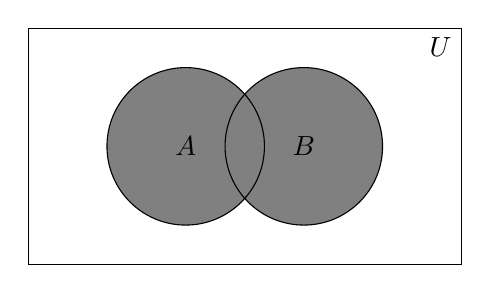
\begin{tikzpicture}
				\draw (-2,-1.5) rectangle (3.5,1.5) node[below left]{$U$};
				\fill[gray] (0,0) circle (1cm);
				\fill[gray] (1.5,0) circle (1cm);
				\draw (0,0) circle (1cm) node {$A$};
				\draw (1.5,0) circle (1cm) node {$B$};
			\end{tikzpicture}
			\caption{$A \cup B$ on a Venn Diagram}
		\end{figure}
		
		\item $A \cap B$ or the \textit{intersection of A and B} is the set containing the element/s that are present in both $A$ and $B$.
		\begin{figure}[!ht]
			\centering
			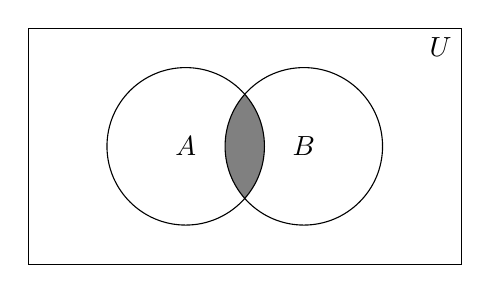
\begin{tikzpicture}
				\draw (-2,-1.5) rectangle (3.5,1.5) node[below left]{$U$};
				\begin{scope}
					\clip (0,0) circle (1cm);
					\fill[gray] (1.5,0) circle (1cm);
				\end{scope}
				\draw (0,0) circle (1cm) node {$A$};
				\draw (1.5,0) circle (1cm) node {$B$};
			\end{tikzpicture}
			\caption{$A \cap B$ on a Venn Diagram}		
		\end{figure}
		
		\item $A$ an $B$ are disjoint sets if they have no same elements. Disjoint sets can be written as $A \cap B=\varnothing$.
		\begin{figure}[!ht]
			\centering
			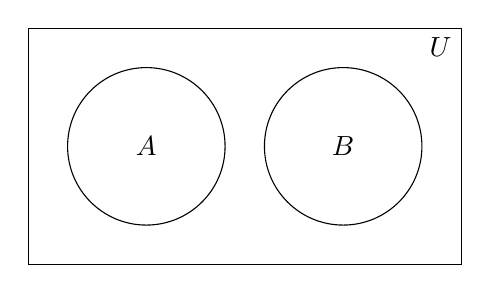
\begin{tikzpicture}
				\draw (-2,-1.5) rectangle (3.5,1.5) node[below left]{$U$};
				\draw (-0.5,0) circle (1cm) node {$A$};
				\draw (2,0) circle (1cm) node {$B$};
			\end{tikzpicture}
			\caption{Disjoint sets $A$ and $B$ on a Venn Diagram}
		\end{figure}
		
		\item $A \setminus B$ or the \textit{set difference of A and B} is the set containing all the elements of $A$ that are not in $B$.
		\begin{itemize}
			\item If $A=B$, then $A \setminus B=\varnothing$.
			\item If $A=\varnothing$, then in any $B$, $A \setminus B=\varnothing$.
		\end{itemize}
		\begin{figure}[!ht]
			\centering
			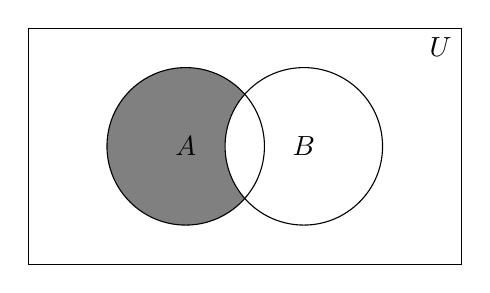
\begin{tikzpicture}
				\draw (-2,-1.5) rectangle (3.5,1.5) node[below left]{$U$};
				\fill[gray] (0,0) circle (1cm);
				\begin{scope}
					\clip (0,0) circle (1cm);
					\fill[white] (1.5,0) circle (1cm);
				\end{scope}
				\draw (0,0) circle (1cm) node {$A$};
				\draw (1.5,0) circle (1cm) node {$B$};
			\end{tikzpicture}
			\caption{$A \setminus B$ on a Venn Diagram}
		\end{figure}
		
		\item $A \Delta B$ or the \textit{symmetric difference of A and B} is  the set containing the elements of set $A$ that are not in set $B$ combined (union) with the set containing the elements of set $B$ that are not in set $A$. It can be written as $(A \setminus B) \cup (B \setminus A)$. 
		
	\end{itemize}
	
	\begin{figure}[!ht]
		\centering
		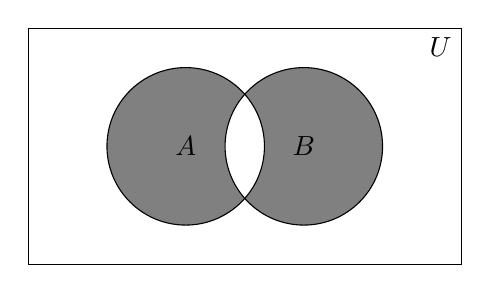
\begin{tikzpicture}
			\draw (-2,-1.5) rectangle (3.5,1.5) node[below left]{$U$};
			\fill[gray] (0,0) circle (1cm);
			\fill[gray] (1.5,0) circle (1cm);
			\begin{scope}
				\clip (0,0) circle (1cm);
				\fill[white] (1.5,0) circle (1cm);
			\end{scope}
			\draw (0,0) circle (1cm) node {$A$};
			\draw (1.5,0) circle (1cm) node {$B$};
		\end{tikzpicture}
		\caption{$A \Delta B$ on a Venn Diagram}
	\end{figure}
	
	\item \textbf{finite set} - a countable set; set that contains countable number elements
	
 	\item  \textbf{cardinality of set $S$ or $|S|$} - the number of elements of set $S$\\
 	Ex. Let $A=\{1,3,5,7,9,11,13,15\}$, then $|A|=8$
 	
 	\item \textbf{power set of $S$ or $P(S)$} - the set that all the possible subsets of S including the empty set\\
 	Ex. Let $B=\{0,1\}$, then $P(B)=\{\varnothing,0,1,01\}$ and $|P(B)|=4$
 	
 	\item Let $k \in \mathbb{N}$ and $a_1,a_2,...,a_k$ are any k number of objects; \textit{ordered k-tuple or k-tuple} can be written as $(a_1,a_2,...,a_k)$.
 	\item Some sets of numbers:
 	\begin{itemize}
 		\item set of natural numbers or $\mathbb{N} = \{1,2,3,...\}$
 		\item integer set or $\mathbb{Z} = \{...,-2,-1,0,1,2,...\}$
 		\item set of rational numbers or $\mathbb{Q} = \{a/b:a,b \in \mathbb{Z},b\neq 0 \}$
 		\item set of real numbers or $\mathbb{R}$
 	\end{itemize}
\end{itemize}

\subsection{Graphs}
\begin{itemize}
	\item \textbf{graph or general graph} - ordered triple $G=(V,E,\phi)$ where, $V\neq\varnothing$, $V \cap E = \varnothing$ and $\phi:E \rightarrow P(V)$ such that $|\phi(e)|={1,2}$ for every $e \in E$.
	
	\item Let G be a graph with $G = (V,E,\phi)$,
		\begin{itemize}
			\item The vertex set or $V$ is the set of vertices of G
			\item The edge set or $E$ is the set of edges
			\item $\phi(e)$ contains the endvertex/endvertices of each $e$ which are the elements of the vertex set. 
		\end{itemize}
	\begin{figure}[!ht]
		\centering
		\begin{tikzpicture}[-,>=stealth',shorten >=1pt,auto,node distance=3cm,thick,main node/.style={circle,draw,font=\sffamily\Large\bfseries}]
			\node[main node] (1) {$v_1$};
			\node[main node] (2) [below left of=1] {$v_2$};
			\node[main node] (3) [below of=1] {$v_3$};
			\node[main node] (4) [below right of=1] {$v_4$};
			\node[main node] (5) [below of=3] {$v_5$};
			\node[main node] (6) [right of=4] {$v_6$};
			\path[every node/.style={font=\sffamily\large}]
				(1) edge node [right] {$e_3$} (4)
					edge node [left] {$e_1$} (2)
					edge node {$e_2$} (3)
				(2) edge [loop left] node {$e_6$} (2)
				(3) edge [bend right] node  {$e_4$} (5)
					edge node [right] {$e_7$} (4)
					edge [bend left,pos=0.2] node  {$e_8$} (5)
				(4) edge node {$e_5$} (5)
				(5) 
				;
		\end{tikzpicture}
		\caption{Graph G with 6 vertices and 7 edges.}
		\label{graph1}
	\end{figure}
	In figure \ref{graph1}, 
	\begin{equation}
		\begin{array}{l}
		G=(V,E,\phi) \\
		V=\{v_1,v_2,v_3,v_4,v_5,v_6\} \\
		E=\{e_1,e_2,e_3,e_4,e_5,e_6,e_7\} \\
		\phi(e_1)=\{v_1,v_2\} \\
		\phi(e_2)=\{v_1,v_3\} \\
		\phi(e_3)=\{v_1,v_4\} \\
		\phi(e_4)=\{v_3,v_5\} \\
		\phi(e_5)=\{v_4,v_5\} \\
		\phi(e_6)=\{v_2\} \\
		\phi(e_7)=\{v_3,v_4\}
		\end{array}
	\end{equation}
	Let the graph $G=(V,E,\phi)$,
	\begin{itemize}
		\item The vertices $u$ and $v$ are in $V$ and are \textit{adjacent/neighbor} of each other , if there is some edge $e \in E$ that has $\phi(e)=\{u,v\}$ or $\{v,u\}$. In figure 1, $v_1$ and $v_2$ are neighbors.
		
		\item The edges $e_1$ and $e_2$ are in $E$ and are \textit{adjacent} if they contain atleast one same end vertex on their respective $\phi$, such that $\phi\{e_1\} \cap \phi\{e_2\} \neq 0$. In figure 1, $e_1$ and $e_2$ are adjacent.
		
		\item Vertex $v$ and edge $e$ are in $V$ and $E$ respectively and are \textit{incident}, if $v$ is in $\phi(e)$. In figure 1, $v_1$ and $e_3$ are incident.

		\item \textbf{Loop} is an edge $e$ with the same endvertices given that $|\phi(e)|=1$. In the figure, $e_2$ is a loop because $\phi(e)=\{v_2\}$
		
		\item $E'$ is a edge set with \textit{multiple/parallel edges}, if $|E'| \leq 2$ and for any edges $e$ and $f$ in $E'$, $\phi(e)=\phi(f)$. In figure, $E'=\{e_4,e_8\}$ because $\phi(e_4)=\phi(e_8)=\{v_3,v_5\}$
		
		\item The vertex $v$ is \textit{isolated} if $v$ is not in $\phi(e)$ for all $e$ in $E$
	\end{itemize}
	
	\item A \textbf{simple graph} is a graph without multiple/parallel edges or loops.
	
	\item A graph $G=(V,E)$ is a simple graph if,
	\begin{enumerate}
		\item $V\neq\varnothing$
		\item $E=\varnothing$
		\item $E=\{\{v_1,v_2\}:v_1,v_2 \in V, v_1 \neq v_2\}$
	\end{enumerate}
	\begin{figure}[!ht]
		\centering
		\begin{tikzpicture}[-,>=stealth',shorten >=1pt,auto,node distance=3cm,thick,main node/.style={circle,draw,font=\sffamily\Large\bfseries}]
		\node[main node] (1) {$v_1$};
		\node[main node] (2) [below left of=1] {$v_2$};
		\node[main node] (3) [below right of=1] {$v_3$};
		\node[main node] (4) [above right of=1] {$v_4$};
  
		\path[every node/.style={font=\sffamily\large}]
			(1) edge node [right] {$e_1$} (2)
			edge node [left] {$e_2$} (3)
			edge node {$e_4$} (4)
			(3) edge node {$e_3$} (4)    
			(4) 
			;
		\end{tikzpicture}
		\caption{An example of simple graph}
	\end{figure}
	
	Some examples of Common graphs:
	\item A graph $G=(V,E)$ is a \textit{null graph} on $n$ vertices if,
		\begin{enumerate}
			\item $V=\{v_1,v_2,...,v_n\}$
			\item $E=\varnothing$
		\end{enumerate}
		\begin{figure}[!ht]
			\centering
			\begin{tikzpicture}[-,>=stealth',shorten >=1pt,auto,node distance=2cm,thick,main node/.style={circle,draw,font=\sffamily\Large\bfseries}]
				\node[main node] (1) {$v_1$};
				\node[main node] (2) [right of=1] {$v_2$};
				\node[main node] (3) [right of=2] {$v_3$};
				\node[main node] (4) [right of=3] {$v_4$};
				;
			\end{tikzpicture}
			\caption{An example of a null graph on 4 vertices}
		\end{figure}
		
	\item A graph $G=(V,E)$ is a \textit{path graph} on $n\geq2$ vertices if,
		\begin{enumerate}
			\item $V=\{v_1,v_2,...,v_n\}$
			\item $E=\{\{u_1,u_2\},\{u_2,u_3\},...,\{u_{n-1},u_{n}\}\}$
		\end{enumerate}
		
		\begin{figure}[!ht]
			\centering
			\begin{tikzpicture}[-,>=stealth',shorten >=1pt,auto,node distance=3cm,thick,main node/.style={circle,draw,font=\sffamily\Large\bfseries}]
				\node[main node] (1) {$v_1$};
				\node[main node] (2) [right of=1] {$v_2$};
				\node[main node] (3) [right of=2] {$v_3$};
				\node[main node] (4) [right of=3] {$v_4$};
  
				\path[every node/.style={font=\sffamily\large}]
				(1) edge node {$e_1$} (2)
				(2) edge node {$e_2$} (3)
				(3) edge node {$e_3$} (4)  
				(4) 
				;
			\end{tikzpicture}
			\caption{An example of a path graph one 4 vertices}
		\end{figure}
		
	\item A graph $G=(V,E)$ is a \textit{cycle graph or cycle} on $n\geq3$ vertices if,
	\begin{enumerate}
		\item $V=\{v_1,v_2,...,v_n\}$
		\item $E=\{\{v_1,v_2\},\{v_2,v_3\},...,\{v_{n-1},v_{n}\},\{v_n,v_1\}\}$
	\end{enumerate}
	\begin{figure}[!ht]
		\centering
		\begin{tikzpicture}[-,>=stealth',shorten >=1pt,auto,node distance=3cm,thick,main node/.style={circle,draw,font=\sffamily\Large\bfseries}]
	  		\node[main node] (1) {$v_1$};
	  		\node[main node] (2) [right of=1] {$v_2$};
	  		\node[main node] (3) [below right of=2] {$v_3$};
	  		\node[main node] (4) [below left of=3] {$v_4$};
	  		\node[main node] (5) [left of=4] {$v_5$};
	  		\node[main node] (6) [above left of=5] {$v_6$};
	  		\path[every node/.style={font=\sffamily\large}]
	  		(1) edge node {$e_1$} (2)
	  		(2) edge node {$e_2$} (3)
	  		(3) edge node {$e_3$} (4)  
	  		(4) edge node {$e_4$} (5)
	  		(5) edge node {$e_5$} (6)
	  		(6) edge node {$e_6$} (1)
	    	;
		\end{tikzpicture}
		\caption{An example of a cycle graph on 6 vertices}
	\end{figure}
	
	\item A graph $G=(V,E)$ is a \textit{complete graph} on $n$ vertices if,
	\begin{enumerate}
		\item $V=\{v_1,v_2,...,v_n\}$
		\item $E=\{\{v_i,v_j\}:1\leq i \leq j \leq n\}$
	\end{enumerate}
	
	\begin{figure}[!ht]
		\centering
		\begin{tikzpicture}[-,>=stealth',shorten >=1pt,auto,node distance=3cm,thick,main node/.style={circle,draw,font=\sffamily\Large\bfseries}]
			\node[main node] (1) {$v_1$};
			\node[main node] (2) [right of=1] {$v_2$};
			\node[main node] (3) [below right of=2] {$v_3$};
			\node[main node] (4) [below left of=3] {$v_4$};
			\node[main node] (5) [left of=4] {$v_5$};
			\node[main node] (6) [above left of=5] {$v_6$};
			\path[every node/.style={font=\sffamily\large}]
			(1) edge node {} (2)
			edge node {} (3)
			edge node {} (4)
			edge node {} (5)
			edge node {} (6)
			(2) edge node {} (3)
			edge node {} (4)
			edge node {} (5)
			edge node {} (6)
			(3) edge node {} (4)
			edge node {} (5)
			edge node {} (6)  
			(4) edge node {} (5)
			edge node {} (6)
			(5) edge node {} (6)
			(6)
			;
		\end{tikzpicture}
		\caption{An example of a complete graph on 6 vertices}
	\end{figure}
	
	\item A graph is a \textit{complete bipartite (m,n)-graph} on $m+n$ vertices, if
	\begin{enumerate}
		\item $V=\{s_1,s_2,...,s_m\} \cup \{v_1,v_2,...,v_n\}$
		\item $E=\{\{s_i,v_j\}:1\leq i \leq m, 1 \leq j \leq n\}$
	\end{enumerate}	
	
	\begin{figure}[!ht]
		\centering
		\begin{tikzpicture}[-,>=stealth',shorten >=1pt,auto,node distance=3cm,                    thick,main node/.style={circle,draw,font=\sffamily\Large\bfseries}]

		  \node[main node] (1) {$v_1$};
		  \node[main node] (2) [right of=1] {$v_2$};
		  \node[main node] (3) [right of=2] {$v_3$};
		  \node[main node] (4) [right of=3] {$v_4$};
		  \node[main node] (5) [below left of=1] {$s_1$};
		  \node[main node] (6) [below right of=1] {$s_2$};
		  \node[main node] (7) [below right of=2] {$s_3$};
		  \node[main node] (8) [below right of=3] {$s_4$};
		  \node[main node] (9) [below right of=4] {$s_5$};
	  
	  \path[every node/.style={font=\sffamily\large}]
	    (1) edge node {} (5)
	    	edge node {} (6)
	    	edge node {} (7)
	    	edge node {} (8)
	    	edge node {} (9)
	    (2) edge node {} (5)
	    	edge node {} (6)
	    	edge node {} (7)
	    	edge node {} (8)
	    	edge node {} (9)
	    (3) edge node {} (5)
	    	edge node {} (6)
	    	edge node {} (7)
	    	edge node {} (8)
	    	edge node {} (9)  
	    (4) edge node {} (5)
	    	edge node {} (6)
	    	edge node {} (7)
	    	edge node {} (8)
	    	edge node {} (9)
	    ;
		\end{tikzpicture}
\caption{An example of a complete bipartite $(4,5)$-graph on $4+5$ vertices}
\end{figure}	 
\end{itemize}
\subsection{Degrees and Regular Graph}
Let $G=(V,E,\phi)$ be a graph with vertex $v\in V$,
\begin{itemize}
	\item $d_G(v)$ or $d(v)$ (when there is no other given graphs) is the \textit{degree of the vertex $v$} given by,
	$$d(v)=|\{e\in E: v \in \phi(e), |\phi(e)|=1,2 \}|$$
	It is the cardinality of edges that are connected to the vertex $v$.\\ 
	Some Remarks:\\  \\
	\begin{tabular}{|l|l|} \hline
		Type of Graph & $d(v)$ \\ \hline
		Simple & number of neighbors of $v$ \\  \hline
		Loopless & number of edges that have $v$ as endvertex \\ \hline
		General & same as loopless but loops are counted twice \\  \hline
	\end{tabular}
	
	\item The set $N_G(v)$ or $N(v)$ is called the \textit{open neighborhood of v} or the \textit{neighborhood of v}.It is the set of all the vertex neighbors of the vertex $v$ in graph $G$. It is given by,
		$$N(v)=\{w \in V: \phi(e)=\{v,w\} or \{w,v\}, e \in E\}$$
		
	\item Additionally, the \textit{closed neighborhood of v}  denoted by $N[v]$  is the set of all the elements in the open neighbor with the vertex $v$ itself. 
	$$N[v]=N(v) \cup v$$
	
	\begin{figure}[!ht]
		\centering
		\begin{tikzpicture}[-,>=stealth',shorten >=1pt,auto,node distance=3cm,thick,main node/.style={circle,draw,font=\sffamily\Large\bfseries}]
	
			\node[main node] (1) {$v_1$};
			\node[main node] (2) [below left of=1] {$v_2$};
			\node[main node] (3) [below right of=1] {$v_3$};
			\node[main node] (4) [right of=3] {$v_4$};
			
			\path[every node/.style={font=\sffamily\large}]
			(1) edge node {} (2)
				edge node {} (3)
			(2) edge [bend left]node {} (3)
				edge [loop left] node {} (2)
			(3) edge [bend left] node {} (2)
				edge node {} (4)
			(4) 
			;
		\end{tikzpicture}
		\caption{An example of a graph with various degrees.}
		\label{degreefig}
	\end{figure}
	
	In figure \ref{degreefig}, 
	\begin{equation}
		\begin{array}{c c}
		d(v_1)=2 & N(v_1)=\{v_2,v_3\} \\
		d(v_2)=5 & N(v_2)=\{v_1,v_3\}\\
		d(v_3)=4 & N(v_3)=\{v_1,v_2,v_4\}\\
		d(v_4)=1 & N(v_4)=\{v_3\}\\
		N[v_1]=N[v_2]=\{v_1,v_2,v_3\} & N[v_3]=V\\
		N[v_4]=\{v_3,v_4\}
		
		\end{array}
	\end{equation}
	
	\item Hand Shake Theorem \\ The \textit{hand shake theorem} was inspired from the hand shaking scenario on a party. Each person in the party needs to shake hands with the other persons in the room. The amount of shake hands made is twice the number of persons in the party. In parallel to graphs, people in the party represents the vertex set of the graph and the shake hands made are the edge set of the graph. The graph $G=(V,E)$ has a total degree of,
 $$\sum\limits_{u\in V} d(v) = 2|E|$$
	
	\item The graph $F=(V',E',\phi')$ is a subset of graph $G=(V,E,\phi)$ if,
	\begin{enumerate}
		\item $V' \subseteq V$,
		\item $E' \subseteq E$,
		\item $\phi'(e) = \phi(e) \forall e \in E'$	
	\end{enumerate}	 
	The subgraph relationship is denoted by $\subseteq$. So that, we can say $F \subseteq G$
	
	\begin{figure}[!ht]
		\centering
		\begin{tikzpicture}[-,>=stealth',shorten >=1pt,auto,node distance=3cm,thick,main node/.style={circle,draw,font=\sffamily\Large\bfseries}]
			\node[main node] (1) {$v_1$};
			\node[main node] (2) [below right of=1] {$v_2$};
			\node[main node] (3) [below left of=1] {$v_3$};
			\node[main node] (4) [above left of=3] {$v_4$};
			\node[main node] (5) [left of=3] {$v_5$};
			
			\path[every node/.style={font=\sffamily\large}]
				(1) edge node {} (2)
			    	edge node {} (4)
			    	edge node {} (5)
			    (2) 
			    (3) edge node {} (4)
			    	edge node {} (5)
			    (4) edge node {} (5)
			    (5)
			    ;
		\end{tikzpicture}
	
		\begin{tikzpicture}[-,>=stealth',shorten >=1pt,auto,node distance=3cm,thick,main node/.style={circle,draw,font=\sffamily\Large\bfseries}]
	
			\node[main node] (1) {$v_1$};
			\node[main node] (3) [below left of=1] {$v_3$};
			\node[main node] (4) [above left of=3] {$v_4$};
			\node[main node] (5) [left of=3] {$v_5$};
	  
			  \path[every node/.style={font=\sffamily\large}]
			    (1)	edge node {} (4)
			    	edge node {} (5)
			    (2) 
			    (3) edge node {} (4)
			    	edge node {} (5)
			    (4) edge node {} (5)
			    (5)
			    ;
		\end{tikzpicture}
		\caption{The graph $F$ (bottom) is a subgraph of graph $G$ (top). }
		\label{subgraphfig}
	\end{figure}
\end{itemize}

\subsection{Directed Graphs}

\begin{itemize}
	\item A \textit{directed graph or digraph} is an ordered triple given by $G=(V,E,\eta)$ where,
	\begin{enumerate}
		\item $V \neq \varnothing$
		\item $V \cap E = \varnothing$
		\item $\eta:E \mapsto V \times V$
	\end{enumerate}
	where, 
	\begin{itemize}
		\item $V$ is the vertex set
		\item $E$ is the set of directed edges
		\item If $u,v \in V$,$e \in E$ and $\eta(e)=(u,v)$, then $u$ is the tail of $e$ and $v$ is the head of $e$.
	\end{itemize}
	
	\begin{figure}[!ht]
		\centering
		\begin{tikzpicture}[->,>=stealth',shorten >=1pt,auto,node distance=3cm,thick,main node/.style={circle,draw,font=\sffamily\Large\bfseries}]
	
		  \node[main node] (1) {$v_1$};
		  \node[main node] (2) [right of=1] {$v_2$};
		  \node[main node] (3) [below left of=2] {$v_3$};
		  \node[main node] (4) [below of=2] {$v_4$};
		  \node[main node] (5) [below of=3] {$v_5$};
		  
		  \path[every node/.style={font=\sffamily\large}]
		    (1) edge node {$e_1$} (2)
		    	
		    (2) edge node {$e_2$} (4)
		    (3) edge node {$e_3$} (2)
		    (4) edge node {$e_4$} (5)
		    (5) edge node {$e_5$} (3)
		    ;
		\end{tikzpicture}
		\caption{An example of a directed graph.}
		\label{digraphfig}
	\end{figure}
	
	In figure \ref{digraphfig}, 
		\begin{equation}
		\begin{array}{c}
		V=\{v_1,v_2,v_3,v_4,v_5\}, \\
		E=\{e_1,e_2,e_3,e_4,e_5\}, \\
		\eta(e_1)=(v_1,v_2), \\
		\eta(e_2)=(v_2,v_4), \\
		\eta(e_3)=(v_3,v_2), \\
		\eta(e_4)=(v_4,v_5), \\
		\eta(e_5)=(v_5,v_3), \\
		\end{array}
		\end{equation}
		
	\item A graph is a \textit{path digraph} on $n\leq2$ vertices, where
	\begin{enumerate}
		\item $V=\{u_1,u_2,...,u_n\}$
		\item $E=\{e_1,e_2,...,e_{n-1}\}$
		\item $\eta(e_1)=(u_i,u_{i+1})$ for all $i \in \{1,...,n-1\}$
	\end{enumerate}
	
	\begin{figure}[!ht]
		\centering
		\begin{tikzpicture}[->,>=stealth',shorten >=1pt,auto,node distance=3cm,thick,main node/.style={circle,draw,font=\sffamily\Large\bfseries}]
		
		  \node[main node] (1) {$v_1$};
		  \node[main node] (2) [above right of=1] {$v_2$};
		  \node[main node] (3) [below right of=2] {$v_3$};
		  \node[main node] (4) [above right of=3] {$v_4$};
		  
		  \path[every node/.style={font=\sffamily\large}]
		    (1) edge node {$e_1$} (2)
		    (2) edge node {$e_2$} (3)
		    (3) edge node {$e_3$} (4)
		    ;
		\end{tikzpicture}
		\caption{An example of a \textit{path digraph on 4 vertices}.}
		\label{pathdigraphfig}
	\end{figure}
	
	\item A graph is a \textit{cycle digraph} on $n\leq1$ vertices, where
	\begin{enumerate}
		\item $V=\{u_1,u_2,...,u_n\}$
		\item $E=\{e_1,e_2,...,e_{n-1},e_n\}$
		\item $\eta(e_1)=(u_i,u_{i+1})$ for all $i \in \{1,...,n-1\}$
		\item $\eta(n)=(u_n,u_1)$
	\end{enumerate}
	
	\begin{figure}[!ht]
		\centering
		\begin{tikzpicture}[->,>=stealth',shorten >=1pt,auto,node distance=3cm,
		                    thick,main node/.style={circle,draw,font=\sffamily\Large\bfseries}]
		
		  \node[main node] (1) {$v_1$};
		  \node[main node] (2) [above right of=1] {$v_2$};
		  \node[main node] (3) [below right of=2] {$v_3$};
		  
		  \path[every node/.style={font=\sffamily\large}]
		    (1) edge node {$e_1$} (2)
		    (2) edge node {$e_2$} (3)
		    (3) edge node {$e_3$} (1)
		    ;
		\end{tikzpicture}
		\caption{An example of a \textit{cycle digraph on 3 vertices}.}
		\label{pathdigraphfig}
	\end{figure}
	
	\item A graph is a \textit{simple digraph} if it has no directed loops and no parallel edges. Figure \ref{digraphfig} is an example of a simple digraph since it has no directed loops and no parallel edges.
\end{itemize}

\subsection{Degrees of Digraph}
Let $G=(V,E,\eta)$ be a digraph and vertex $u \in V$ ,
\begin{itemize}
	\item The \textit{indegree of u} denoted by $d_G^-(u)$ or $d^-(u)$ is the number of directed edges having $u$ as a head, that is,\\
	\begin{center}
	$d^-(u)=|\{e \in E: \eta(e)=(x,u)$ for some $ x \in V\}|$
	\end{center}
	
	\item The \textit{outdegree of u} denoted by $d_G^+(u)$ or $d^+(u)$ is the number of directed edges having $u$ as a head, that is,\\
	\begin{center}
	$d^+(u)=|\{e \in E: \eta(e)=(u,y)$ for some $ y \in V\}|$
	\end{center}
	
	\item The \textit{inneighbors of u} denoted by $N_G^-$ or $N^-$ is given by,
	\begin{center}
	$N^-(u)=\{x \in V: \eta(e)=(x,u)$ for some $ e \in E\}$
	\end{center}
	
	\item The \textit{outneighbors of u} denoted by $N_G^+$ or $N^+$ is given by,
	\begin{center}
	$N^+(u)=\{x \in V: \eta(e)=(u,y)$ for some $ e \in E\}$
	\end{center}
	
	\item 
	\begin{center}
		$\sum\limits_{u\in V} d^-(u) = \sum\limits_{u\in V} d^+(u)=|E|$
	\end{center}
\end{itemize}

\subsection{Paths, Cycles and Weights}
Let $G=(V,E,\phi)$ be a graph with $V=\{v_1,v_2,...,v_k\}$ and $E=\{e_1,e_2,...,e_k\}$ as its vertex and edge set respectively, then,
\begin{enumerate}
	\item A \textbf{walk} in graph G is the alternating sequence of edges and vertices that start and stops with a vertex given by,
	$(v_1,e_1,v_2,e_2,...,e_k,v_k)$ such that $\phi(e_j)=\{v_{j-1},v_j\}$ for $j \in k$.
	
	\item A trail in G is a walk with all of its edges to be distinct.
	
	\item A path in G is a walk with all of its vertices to be distinct.
	
	\item A $u-v$ walk/trail/path is a walk starting from  the vertex $u$ and ends on the vertex $v$ with their respective characteristics.
	
	\item A $v-v$ walk/trail is a circuit (or closed walk/trail).
	
	\item A $v-v$ path is a cycle.\\
	
	\begin{figure}[!ht]
		\centering
		\begin{tikzpicture}[-,>=stealth',shorten >=1pt,auto,node distance=3cm,
	                    thick,main node/.style={circle,draw,font=\sffamily\Large\bfseries}]
	
		  \node[main node] (1) {$v_1$};
		  \node[main node] (2) [right of=1] {$v_2$};
		  \node[main node] (3) [below left of=1] {$v_3$};
		  \node[main node] (4) [right of=2] {$v_4$};
		  \node[main node] (5) [below right of=3] {$v_5$};
		  \node[main node] (6) [right of=5] {$v_6$};
		  
		  \path[every node/.style={font=\sffamily\large}]
		    (1) edge node {$e_1$} (2)
		    	edge [bend left] node {$e_2$} (3)
		    	edge node {$e_3$} (5)
		    	edge node {$e_4$} (6)
		    (2) edge node {$e_5$} (4)
		    (3) edge node {$e_6$} (5)
		    	edge [bend left] node{$e_7$} (1)
		    (4) edge node {$e_8$} (6)
		    (5) edge node {$e_9$} (6)
		    (6)
		    ;
		\end{tikzpicture}
		\caption{An example of a graph to show walks,trails,paths and cycles.}
		\label{walkfig}
	\end{figure}
	
	\item In figure \ref{walkfig},
	\begin{itemize}
		\item $q=(v_1,e_2,v_3,e_7,v_1,e_4,v_6,e_4,v_1,e_1,v_2,e_5,v_4)$\\ $q$ is a walk of length 6. $q$ is not a trail since $e_4$ is repeated. $q$ is not also a path because $v_1$ appeared many times.
		
		\item $r=(v_3,e_2,v_1,e_7,v_3,e_6,v_5,e_9,v_6,e_8,v_4)$ \\ $r$ is a walk of length 5 and a trail because there are no repeating edges. $r$ is no a path because the vertex $v_3$ is repeated.
		
		\item $t=(v_1,e_1,v_2,e_5,v_4,e_8,v_6,e_9,v_5)$ \\ $t$ is a path of length 4 because there are no repeating vertices in the walk.
		
		\item $d=(v_1,e_1,v_2,e_5,v_4,e_8,v_6,e_9,v_5,e_3,v_1)$ \\ $d$ is a closed walk, closed trail and a cycle of length 5.
	\end{itemize}
	
	\item Let $G$ be a graph and $W: E \rightarrow \mathbb{R}$, the ordered tuple $(G,W)$ is called a \textit{weighted graph}. The function $W$ is called a \textit{weight/weight function} of $(G,W)$.
	
	\begin{figure}[!ht]
		\centering
		\begin{tikzpicture}[->,>=stealth',shorten >=1pt,auto,node distance=3cm,thick,main node/.style={circle,draw,font=\sffamily\Large\bfseries}]
		
		  \node[main node] (1) {$v_1$};
		  \node[main node] (2) [below left of=1] {$v_2$};
		  \node[main node] (3) [below right of=1] {$v_3$};
		  \node[main node] (4) [above right of=1] {$v_4$};
		  
		  \path[every node/.style={font=\sffamily\large}]
		    (1) edge node [right] {$1.2$} (2)
		    	edge node [left] {$0.6$} (3)
		    	edge node {$1.33$} (4)
		    (2) 
		    (3) edge node {$0.4$} (4)
		        
		    (4) 
		    ;
		\end{tikzpicture}
		\caption{An example of a weighted simple digraph}
		\label{wgraph}
	\end{figure}
	
	In figure \ref{wgraph},
	\begin{equation}
		\begin{array}{c}
			W((v_1,v_2))=1.2\\
			W((v_1,v_3))=0.6\\
			W((v_1,v_4))=1.33\\
			W((v_3,v_4))=0.4
		\end{array}
	\end{equation}
\end{enumerate}

%\subsection{Connectivity, Isomorphism and Homomorphism}
%\begin{itemize}
%	\item A graph $G=(V,E,\phi)$ is \textit{connected} if, for every unique pair vertices $u,v \in V$, $G$ has a $u,v$-path. Otherwise, $G$ is \textit{disconnected}.
%	\item Let $G=(V,E,\phi)$ and $G'=(V',E',\phi')$ be graphs. A \textit{homomorphism} $f:G \rightarrow G'$ from $G$ to $G'$ is an ordered pair $f=(f_1,f_2)$ of maps, $f_1:V \rightarrow V'$ and $f_2=E \rightarrow E'$, also satisfying the compatibility condition, $$\phi(e)=\{u,v\} \implies \phi'(f_2(e))= \{f_1(u),f_1(v)\} $$
%	So if $u$ and $v$ are envertices of an edge $e$ in $G$, then $f_1(u)$ and $f_21(v)$ must also be the end vertices of edge $f_2(e)$ in $G'$.
%\end{itemize}